\begin{figure}[H]
	\centering
	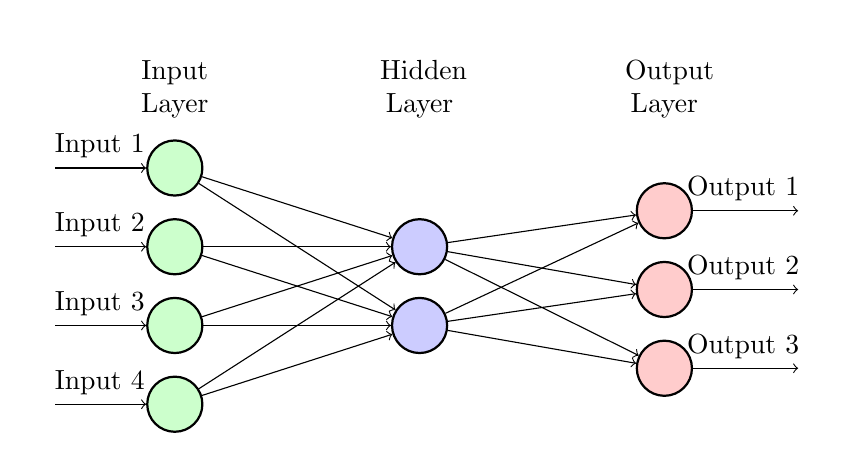
\begin{tikzpicture}[
		->,
		input node/.style={circle, draw, thick, fill=green!20,minimum size = 7mm},
		hidden node/.style={circle, draw, thick, fill=blue!20,minimum size = 7mm},
		output node/.style={circle, draw, thick, fill=red!20,minimum size = 7mm},
		dummy node/.style={circle, thick}
	]
		\node[dummy node] (d1) {};
		\node[dummy node,below of=d1] (d2) {};
		\node[dummy node,below of=d2] (d3) {};
		\node[dummy node,below of=d3] (d4) {};

		\node[input node,right of=d1,xshift=20pt] (i1) {};
		\node[input node,below of=i1] (i2) {};
		\node[input node,below of=i2] (i3) {};
		\node[input node,below of=i3] (i4) {};

		\node[hidden node,right of=i2,xshift=60pt] (h1) {};
		\node[hidden node,right of=i3,xshift=60pt] (h2) {};

		\node[output node,right of=h1,yshift=13pt,xshift=60pt] (o1) {};
		\node[output node,below of=o1] (o2) {};
		\node[output node,below of=o2] (o3) {};

		\node[dummy node,right of=o1, xshift=25pt] (do1) {};
		\node[dummy node,below of=do1] (do2) {};
		\node[dummy node,below of=do2] (do3) {};

		\foreach \i in {1,...,4} {
			\draw[<-] (i\i) -- (d\i) node[above,xshift=0.75cm] {Input \i};
		}

		\foreach \i in {1,...,4} {
			\foreach \h in {1,...,2} {
				\draw[->] (i\i) -- (h\h) {};
			}
		}

		\foreach \h in {1,...,2} {
			\foreach \o in {1,...,3} {
				\draw[->] (h\h) -- (o\o) {};
			}
		}

		\foreach \o in {1,...,3} {
			\draw[<-] (do\o) -- (o\o) node[above,xshift=1cm] {Output \o};
		}

		\node[dummy node, above of=i1,text width=1cm, align=center] (lin) {Input Layer};
		\node[dummy node, right of=lin,text width=1cm,align=center, xshift=60pt] (lhi) {Hidden Layer};
		\node[dummy node, right of=lhi,text width=1cm,align=center, xshift=60pt] (lou) {Output Layer};

		
	\end{tikzpicture}
	\caption{Una rete neurale con un solo livello nascosto.}
	\label{fig:nnet}
\end{figure}
